\documentclass[a4paper,12pt]{article}

%%% HarrixLaTeXDocumentTemplate
%%% Версия 1.16
%%% Шаблон документов в LaTeX на русском языке. Данный шаблон применяется в проектах HarrixTestFunctions, MathHarrixLibrary, Standard-Genetic-Algorithm  и др.
%%% https://github.com/Harrix/HarrixLaTeXDocumentTemplate
%%% Шаблон распространяется по лицензии Apache License, Version 2.0.

%%% Поля и разметка страницы %%%
\usepackage{lscape} % Для включения альбомных страниц
\usepackage{geometry} % Для последующего задания полей

%%% Кодировки и шрифты %%%
\usepackage{pscyr} % Нормальные шрифты
\usepackage{cmap} % Улучшенный поиск русских слов в полученном pdf-файле
\usepackage[T2A]{fontenc} % Поддержка русских букв
\usepackage[utf8]{inputenc} % Кодировка utf8
\usepackage[english, russian]{babel} % Языки: русский, английский

%%% Математические пакеты %%%
\usepackage{amsthm,amsfonts,amsmath,amssymb,amscd} % Математические дополнения от AMS
%%% Для жиного курсива в формулах %%%
\usepackage{bm}

%%% Оформление абзацев %%%
\usepackage{indentfirst} % Красная строка
\usepackage{setspace} % Расстояние между строками
\usepackage{enumitem} % Для список обнуление расстояния до абзаца

%%% Цвета %%%
\usepackage[usenames]{color}
\usepackage{color}
\usepackage{colortbl}

%%% Таблицы %%%
\usepackage{longtable} % Длинные таблицы
\usepackage{multirow,makecell,array} % Улучшенное форматирование таблиц

%%% Общее форматирование
\usepackage[singlelinecheck=off,center]{caption} % Многострочные подписи
\usepackage{soul} % Поддержка переносоустойчивых подчёркиваний и зачёркиваний

%%% Библиография %%%
\usepackage{cite}

%%% Гиперссылки %%%
\usepackage{hyperref}

%%% Изображения %%%
\usepackage{graphicx} % Подключаем пакет работы с графикой
\usepackage{epstopdf}
\usepackage{subcaption}

%%% Отображение кода %%%
\usepackage{xcolor}
\usepackage{listings}
\usepackage{caption}

%%% Псевдокоды %%%
\usepackage{algorithm} 
\usepackage{algpseudocode}

%%% Рисование графиков %%%
\usepackage{pgfplots}

%%% Макет страницы %%%
\geometry{a4paper,top=2cm,bottom=2cm,left=2cm,right=1cm}

%%% Кодировки и шрифты %%%
%\renewcommand{\rmdefault}{ftm} % Включаем Times New Roman

%%% Выравнивание и переносы %%%
\sloppy
\clubpenalty=10000
\widowpenalty=10000

%%% Библиография %%%
\makeatletter
\bibliographystyle{utf8gost705u} % Оформляем библиографию в соответствии с ГОСТ 7.0.5
\renewcommand{\@biblabel}[1]{#1.} % Заменяем библиографию с квадратных скобок на точку:
\makeatother

%%% Изображения %%%
\graphicspath{{images/}} % Пути к изображениям
% Поменять двоеточние на точку в подписях к рисунку
\RequirePackage{caption}
\DeclareCaptionLabelSeparator{defffis}{. }
\captionsetup{justification=centering,labelsep=defffis}

%%% Цвета %%%
% Цвета для кода
\definecolor{string}{HTML}{B40000} % цвет строк в коде
\definecolor{comment}{HTML}{008000} % цвет комментариев в коде
\definecolor{keyword}{HTML}{1A00FF} % цвет ключевых слов в коде
\definecolor{morecomment}{HTML}{8000FF} % цвет include и других элементов в коде
\definecolor{сaptiontext}{HTML}{FFFFFF} % цвет текста заголовка в коде
\definecolor{сaptionbk}{HTML}{999999} % цвет фона заголовка в коде
\definecolor{bk}{HTML}{FFFFFF} % цвет фона в коде
\definecolor{frame}{HTML}{999999} % цвет рамки в коде
\definecolor{brackets}{HTML}{B40000} % цвет скобок в коде
% Цвета для гиперссылок
\definecolor{linkcolor}{HTML}{799B03} % цвет ссылок
\definecolor{urlcolor}{HTML}{799B03} % цвет гиперссылок
\definecolor{citecolor}{HTML}{799B03} % цвет гиперссылок
\definecolor{gray}{rgb}{0.4,0.4,0.4}
\definecolor{darkblue}{rgb}{0.0,0.0,0.6}

%%% Отображение кода %%%
% Настройки отображения кода
\lstset{
language=C++, % Язык кода по умолчанию
morekeywords={*,...}, % если хотите добавить ключевые слова, то добавляйте
% Цвета
keywordstyle=\color{keyword}\ttfamily\bfseries,
%stringstyle=\color{string}\ttfamily,
stringstyle=\ttfamily\color{red!50!brown},
commentstyle=\color{comment}\ttfamily\itshape,
morecomment=[l][\color{morecomment}]{\#}, 
% Настройки отображения     
breaklines=true, % Перенос длинных строк
basicstyle=\ttfamily\footnotesize, % Шрифт для отображения кода
backgroundcolor=\color{bk}, % Цвет фона кода
frame=lrb,xleftmargin=\fboxsep,xrightmargin=-\fboxsep, % Рамка, подогнанная к заголовку
rulecolor=\color{frame}, % Цвет рамки
tabsize=3, % Размер табуляции в пробелах
% Настройка отображения номеров строк. Если не нужно, то удалите весь блок
%numbers=left, % Слева отображаются номера строк
%stepnumber=1, % Каждую строку нумеровать
%numbersep=5pt, % Отступ от кода 
%numberstyle=\small\color{black}, % Стиль написания номеров строк
% Для отображения русского языка
extendedchars=true,
literate={Ö}{{\"O}}1
  {Ä}{{\"A}}1
  {Ü}{{\"U}}1
  {ß}{{\ss}}1
  {ü}{{\"u}}1
  {ä}{{\"a}}1
  {ö}{{\"o}}1
  {~}{{\textasciitilde}}1
  {а}{{\selectfont\char224}}1
  {б}{{\selectfont\char225}}1
  {в}{{\selectfont\char226}}1
  {г}{{\selectfont\char227}}1
  {д}{{\selectfont\char228}}1
  {е}{{\selectfont\char229}}1
  {ё}{{\"e}}1
  {ж}{{\selectfont\char230}}1
  {з}{{\selectfont\char231}}1
  {и}{{\selectfont\char232}}1
  {й}{{\selectfont\char233}}1
  {к}{{\selectfont\char234}}1
  {л}{{\selectfont\char235}}1
  {м}{{\selectfont\char236}}1
  {н}{{\selectfont\char237}}1
  {о}{{\selectfont\char238}}1
  {п}{{\selectfont\char239}}1
  {р}{{\selectfont\char240}}1
  {с}{{\selectfont\char241}}1
  {т}{{\selectfont\char242}}1
  {у}{{\selectfont\char243}}1
  {ф}{{\selectfont\char244}}1
  {х}{{\selectfont\char245}}1
  {ц}{{\selectfont\char246}}1
  {ч}{{\selectfont\char247}}1
  {ш}{{\selectfont\char248}}1
  {щ}{{\selectfont\char249}}1
  {ъ}{{\selectfont\char250}}1
  {ы}{{\selectfont\char251}}1
  {ь}{{\selectfont\char252}}1
  {э}{{\selectfont\char253}}1
  {ю}{{\selectfont\char254}}1
  {я}{{\selectfont\char255}}1
  {А}{{\selectfont\char192}}1
  {Б}{{\selectfont\char193}}1
  {В}{{\selectfont\char194}}1
  {Г}{{\selectfont\char195}}1
  {Д}{{\selectfont\char196}}1
  {Е}{{\selectfont\char197}}1
  {Ё}{{\"E}}1
  {Ж}{{\selectfont\char198}}1
  {З}{{\selectfont\char199}}1
  {И}{{\selectfont\char200}}1
  {Й}{{\selectfont\char201}}1
  {К}{{\selectfont\char202}}1
  {Л}{{\selectfont\char203}}1
  {М}{{\selectfont\char204}}1
  {Н}{{\selectfont\char205}}1
  {О}{{\selectfont\char206}}1
  {П}{{\selectfont\char207}}1
  {Р}{{\selectfont\char208}}1
  {С}{{\selectfont\char209}}1
  {Т}{{\selectfont\char210}}1
  {У}{{\selectfont\char211}}1
  {Ф}{{\selectfont\char212}}1
  {Х}{{\selectfont\char213}}1
  {Ц}{{\selectfont\char214}}1
  {Ч}{{\selectfont\char215}}1
  {Ш}{{\selectfont\char216}}1
  {Щ}{{\selectfont\char217}}1
  {Ъ}{{\selectfont\char218}}1
  {Ы}{{\selectfont\char219}}1
  {Ь}{{\selectfont\char220}}1
  {Э}{{\selectfont\char221}}1
  {Ю}{{\selectfont\char222}}1
  {Я}{{\selectfont\char223}}1
  {і}{{\selectfont\char105}}1
  {ї}{{\selectfont\char168}}1
  {є}{{\selectfont\char185}}1
  {ґ}{{\selectfont\char160}}1
  {І}{{\selectfont\char73}}1
  {Ї}{{\selectfont\char136}}1
  {Є}{{\selectfont\char153}}1
  {Ґ}{{\selectfont\char128}}1
  {\{}{{{\color{brackets}\{}}}1 % Цвет скобок {
  {\}}{{{\color{brackets}\}}}}1 % Цвет скобок }
}
% Для настройки заголовка кода
\DeclareCaptionFont{white}{\color{сaptiontext}}
\DeclareCaptionFormat{listing}{\parbox{\linewidth}{\colorbox{сaptionbk}{\parbox{\linewidth}{#1#2#3}}\vskip-4pt}}
\captionsetup[lstlisting]{format=listing,labelfont=white,textfont=white}
\renewcommand{\lstlistingname}{Код} % Переименование Listings в нужное именование структуры
% Для отображения кода формата xml
\lstdefinelanguage{XML}
{
  morestring=[s]{"}{"},
  morecomment=[s]{?}{?},
  morecomment=[s]{!--}{--},
  commentstyle=\color{comment},
  moredelim=[s][\color{black}]{>}{<},
  moredelim=[s][\color{red}]{\ }{=},
  stringstyle=\color{string},
  identifierstyle=\color{keyword}
}

%%% Гиперссылки %%%
\hypersetup{pdfstartview=FitH,  linkcolor=linkcolor,urlcolor=urlcolor,citecolor=citecolor, colorlinks=true}

%%%  Оформление абзацев %%%
\setlength{\parskip}{0.3cm} % отступы между абзацами
% оформление списков
\setlist{leftmargin=1.5cm,topsep=0pt}

%%% Псевдокоды %%%
% Добавляем свои блоки
\makeatletter
\algblock[ALGORITHMBLOCK]{BeginAlgorithm}{EndAlgorithm}
\algblock[BLOCK]{BeginBlock}{EndBlock}
\makeatother

% Нумерация блоков
\usepackage{caption}% http://ctan.org/pkg/caption
\captionsetup[ruled]{labelsep=period}
\makeatletter
\@addtoreset{algorithm}{chapter}% algorithm counter resets every chapter
\makeatother
\renewcommand{\thealgorithm}{\thechapter.\arabic{algorithm}}% Algorithm # is <chapter>.<algorithm>

%%% Формулы %%%
%Дублирование символа при переносе
\newcommand{\hm}[1]{#1\nobreak\discretionary{}{\hbox{\ensuremath{#1}}}{}}

%%% Таблицы %%%
% Раздвигаем в таблице без границ отступы между строками вновой команде
\newenvironment{tabularwide}%
{\setlength{\extrarowheight}{0.3cm}\begin{tabular}{  p{\dimexpr 0.45\linewidth-2\tabcolsep} p{\dimexpr 0.55\linewidth-2\tabcolsep}  }}  {\end{tabular}}
\newenvironment{tabularwide08}%
{\setlength{\extrarowheight}{0.3cm}\begin{tabular}{  p{\dimexpr 0.8\linewidth-2\tabcolsep} p{\dimexpr 0.2\linewidth-2\tabcolsep}  }}  {\end{tabular}}
% Многострочная ячейка в таблице
\newcommand{\specialcell}[2][c]{%
  {\renewcommand{\arraystretch}{1}\begin{tabular}[t]{@{}l@{}}#2\end{tabular}}}

\newcommand{\specialcelltwoin}[2][c]{%
  {\renewcommand{\arraystretch}{1}\begin{tabular}[t]{@{}b{2in}}#2\end{tabular}}}
  
%%% Абзацы %%
% Отсупы между строками
\singlespacing

\title{Описание множества операторов для алгоритмов оптимизации. v. 1.0}
\author{А.\,Б. Сергиенко}
\date{\today}


\begin{document}

%%% HarrixLaTeXDocumentTemplate
%%% Версия 1.11
%%% Шаблон документов в LaTeX на русском языке. Данный шаблон применяется в проектах HarrixTestFunctions, MathHarrixLibrary, Standard-Genetic-Algorithm  и др.
%%% https://github.com/Harrix/HarrixLaTeXDocumentTemplate
%%% Шаблон распространяется по лицензии Apache License, Version 2.0.

%%% Именования %%%
\renewcommand{\abstractname}{Аннотация}
\renewcommand{\alsoname}{см. также}
\renewcommand{\appendixname}{Приложение}
\renewcommand{\bibname}{Литература}
\renewcommand{\ccname}{исх.}
\renewcommand{\chaptername}{Глава}
%\renewcommand{\contentsname}{Содержание}
\renewcommand{\enclname}{вкл.}
\renewcommand{\figurename}{Рисунок}
\renewcommand{\headtoname}{вх.}
\renewcommand{\indexname}{Предметный указатель}
\renewcommand{\listfigurename}{Список рисунков}
\renewcommand{\listtablename}{Список таблиц}
\renewcommand{\pagename}{Стр.}
\renewcommand{\partname}{Часть}
\renewcommand{\refname}{Список литературы}
\renewcommand{\seename}{см.}
\renewcommand{\tablename}{Таблица}

%%% Псевдокоды %%%
% Перевод данных об алгоритмах
\renewcommand{\listalgorithmname}{Список алгоритмов}
\floatname{algorithm}{Алгоритм}

% Перевод команд псевдокода
\algrenewcommand\algorithmicwhile{\textbf{До тех пока}}
\algrenewcommand\algorithmicdo{\textbf{выполнять}}
\algrenewcommand\algorithmicrepeat{\textbf{Повторять}}
\algrenewcommand\algorithmicuntil{\textbf{Пока выполняется}}
\algrenewcommand\algorithmicend{\textbf{Конец}}
\algrenewcommand\algorithmicif{\textbf{Если}}
\algrenewcommand\algorithmicelse{\textbf{иначе}}
\algrenewcommand\algorithmicthen{\textbf{тогда}}
\algrenewcommand\algorithmicfor{\textbf{Цикл. }}
\algrenewcommand\algorithmicforall{\textbf{Выполнить для всех}}
\algrenewcommand\algorithmicfunction{\textbf{Функция}}
\algrenewcommand\algorithmicprocedure{\textbf{Процедура}}
\algrenewcommand\algorithmicloop{\textbf{Зациклить}}
\algrenewcommand\algorithmicrequire{\textbf{Условия:}}
\algrenewcommand\algorithmicensure{\textbf{Обеспечивающие условия:}}
\algrenewcommand\algorithmicreturn{\textbf{Возвратить}}
\algrenewtext{EndWhile}{\textbf{Конец цикла}}
\algrenewtext{EndLoop}{\textbf{Конец зацикливания}}
\algrenewtext{EndFor}{\textbf{Конец цикла}}
\algrenewtext{EndFunction}{\textbf{Конец функции}}
\algrenewtext{EndProcedure}{\textbf{Конец процедуры}}
\algrenewtext{EndIf}{\textbf{Конец условия}}
\algrenewtext{EndFor}{\textbf{Конец цикла}}
\algrenewtext{BeginAlgorithm}{\textbf{Начало алгоритма}}
\algrenewtext{EndAlgorithm}{\textbf{Конец алгоритма}}
\algrenewtext{BeginBlock}{\textbf{Начало блока. }}
\algrenewtext{EndBlock}{\textbf{Конец блока}}
\algrenewtext{ElsIf}{\textbf{иначе если }}

\maketitle

\begin{abstract}
В данном документе дано собрано множество всяких операторов, которые используются автором в своих исследований. В первую очередь это операторы модификаций генетического алгоритма, а также классические операторы алгоритма.
\end{abstract}

\tableofcontents

\newpage

\section{Введение}

Это своеобразная <<свалка>> операторов, которые используются автором. На данный документ можно ссылаться в своих работах, чтобы указать, что та или иная модификация операторов подробно описана в этом документе. Тут нет исследований эффективности алгоритмов с данными операторами --- это задача иных проектов. Здесь представлено только описание операторов.

Например, в работе может быть написано следующее: <<Модифицированный генетический алгоритм основан на стандартном генетическом алгоритме (\href{https://github.com/Harrix/Standard-Genetic-Algorithm}{https://github.com/Harrix/Standard-Genetic-Algorithm}). Предложенный алгоритм отличается только оператором скрещивания, и вместо двухточечного скрещивания используется двухточечное скрещивание с возможностью точек разрыва по краям хромосомы (подробное описание смотрите в \href{https://github.com/Harrix/HarrixSetOfOperatorsAlgorithms}{https://github.com/Harrix/HarrixSetOfOperatorsAlgorithms})>>.

Данный документ представляет его версию 1.0 от \today

Последнюю версию документа можно найти по адресу:

\href{https://github.com/Harrix/HarrixSetOfOperatorsAlgorithms}{https://github.com/Harrix/HarrixSetOfOperatorsAlgorithms}

С автором можно связаться по адресу \href{mailto:sergienkoanton@mail.ru}{sergienkoanton@mail.ru} или  \href{http://vk.com/harrix}{http://vk.com/harrix}.

Сайт автора, где публикуются последние новости: \href{http://blog.harrix.org/}{http://blog.harrix.org/}, а проекты располагаются по адресу \href{http://harrix.org/}{http://harrix.org/}.

\section{Условные обозначения}\label{SetOfOperatorsAlgorithms:section_symbols}

$a \in A$ --- элемент $ a $ принадлежит множеству $ A $.

$ \bar{x} $ --- обозначение вектора.

$ \arg{f(x)} $ --- возвращает аргумент $x$, при котором функция принимает значение $ f(x) $.

$ Random(X) $ --- случайный выбор элемента из множества $ X $ с равной вероятностью.

$ Random\left ( \left \{x^i \mid p^i \right \} \right ) $ --- случайный выбор элемента $ x^i $ из множества $ X $, при условии, что каждый элемент $ x^i\in X $ имеет вероятность выбора равную $ p^i $, то есть это обозначение равнозначно предыдущему.

$ random(a,b) $ --- случайное действительное число из интервала $ [a; b] $.

$ int(a) $ --- целая часть действительного числа $ a $.

$ \mu(X) $ --- мощность множества $ X $.

\textbf{Замечание.} Оператор присваивания обозначается через знак «$ = $», так же как и знак равенства.

\textbf{Замечание.} Индексация всех массивов в документе начинается с $ 1 $. Это стоит помнить при реализации алгоритма на C-подобных языках программирования, где индексация начинается с нуля.

\textbf{Замечание.} Вызывание трех функций: $ Random(X) $, $ Random\left ( \left \{x_i \mid p_i \right \} \right ) $, $ random(a,b) $ – происходит каждый раз, когда по ходу выполнения формул, они встречаются. Если формула итерационная, то нельзя перед ее вызовом один раз определить, например, $ random(a,b) $ как константу и потом её использовать на протяжении всех итераций неизменной.

\textbf{Замечание.} Надстрочный индекс может обозначать как возведение в степень, так и индекс элемента. Конкретное обозначение определяется в контексте текста, в котором используется формула с надстрочным индексом. 

\textbf{Замечание.} Если у нас имеется множество векторов, то подстрочный индекс обозначает номер компоненты конкретного вектора, а надстрочный индекс обозначает номер вектора во множестве, например, $ \bar{x}^i \in X $ ($i=\overline{1,N}$), $ \bar{x}^i_j \in \left\lbrace 0; 1\right\rbrace  $, ($j=\overline{1,n}$). В случае, если вектор имеет свое обозначение в виде подстрочной надписи, то компоненты вектора проставляются за скобками, например, $ \left( \bar{x}_{max}\right)_j=0$ ($j=\overline{1,n}$). 

\textbf{Замечание.} При выводе матриц и векторов элементы могут разделяться как пробелом, так и точкой с запятой, то есть обе записи $ {\left(\begin{array}{cccccccc}
 1&1&1&1&1&1&1&1
\end{array} \right)}^\mathrm{T} $ и $ {\left(1;1;1;1;1;1;1;1;1 \right)}^\mathrm{T} $ допустимы.

\textbf{Замечание.} При выводе множеств элементы разделяются только точкой с запятой, то есть допустима только такая запись: $ {\left\lbrace 1;1;1;1;1;1;1;1;1 \right\rbrace }^\mathrm{T} $.

\section{Операторы селекции}\label{SetOfOperatorsAlgorithms:section_selection}

Селекция --- оператор случайного выбора одного индивида из популяции, основываясь на значениях функции пригодности всех индивидов текущей популяции, для использования его в операторе скрещивания. При этом вероятность выбора у индивидов с более высокой пригодностью выше, чем у индивидов с более низкой пригодностью.

\subsection{Пропорциональная селекция}\label{SetOfOperatorsAlgorithms:ProportionalSelection}

Идентификатор: \textbf{ProportionalSelection}.

Вероятность выбора элемента пропорциональна значению пригодности индивида. Данный вид селекции может работать только с неотрицательными значениями пригодности.

Пропорциональная селекция определяется формулой:

\begin{equation}
\label{SetOfOperatorsAlgorithms:eq:ProportionalSelection}
Selection\left( Population, Fitness, DataOfSel\right) = Random\left( \left\lbrace\bar{x}^i | p^i \right\rbrace \right),
\end{equation}
\begin{equation}
p^i=\left\lbrace \begin{aligned}
\dfrac{f_{fit}\left( \bar{x}^i\right) }{\sum_{j=1}^N{f_{fit}\left( \bar{x}^j\right)}},&\text { если }  \exists f_{fit}\left( \bar{x}^k\right)\neq 0 \left( k=\overline{1,N} \right); \\ \dfrac{1}{N} ,&\text { иначе}.
\end{aligned}\right.
\end{equation}

где $ \bar{x}^i \in Population, i=\overline{1,N} $.

Как видим, формула определения вероятности выбора индивида имеет составной вид. Второе условие предназначено для маловероятного случая, когда в популяции все индивиды будут иметь пригодность равную нулю.

\textbf{Пример.} Пусть $ Fitness=\left\lbrace 0,5; 0,2; 0,1; 0,6; 0,2; 0,4\right\rbrace $. Тогда вероятности выбора индивидов равны:
\begin{flalign*}
p_1&=\frac{0,5}{0,5 + 0,2 + 0,1 + 0,6 + 0,2 + 0,4}=0,25;\\
p_2&=\frac{0,2}{0,5 + 0,2 + 0,1 + 0,6 + 0,2 + 0,4}=0,1;\\
p_3&=\frac{0,1}{0,5 + 0,2 + 0,1 + 0,6 + 0,2 + 0,4}=0,05;\\
p_4&=\frac{0,6}{0,5 + 0,2 + 0,1 + 0,6 + 0,2 + 0,4}=0,3;\\
p_5&=\frac{0,2}{0,5 + 0,2 + 0,1 + 0,6 + 0,2 + 0,4}=0,1;\\
p_6&=\frac{0,4}{0,5 + 0,2 + 0,1 + 0,6 + 0,2 + 0,4}=0,2.
\end{flalign*}

\begin{figure} [H] 
  \center
  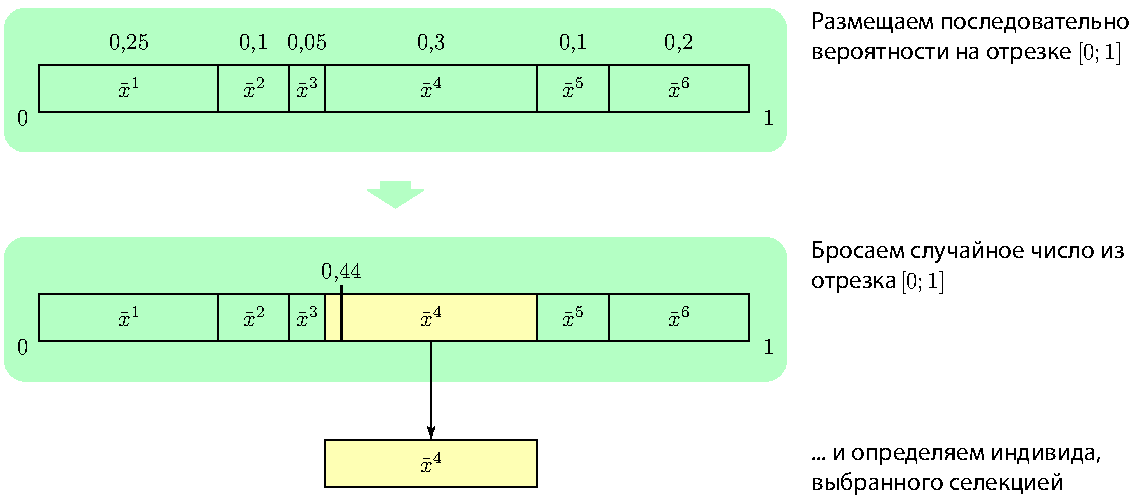
\includegraphics [scale=0.7] {ProportionalSelection}
  \caption{Механизм работы пропорциональной селекции} 
  \label{SetOfOperatorsAlgorithms:img:ProportionalSelection}  
\end{figure}

$ DataOfSel $ также не содержит каких-либо параметров относительно данного типа селекции.

Нет ограничений на множество задач оптимизации, которые может решать алгоритм оптимизации с данной селекцией. 

В библиотеке \textbf{HarrixMathLibrary} данная селекция реализуется через функции \textbf{MHL\_ProportionalSelection}, \textbf{MHL\_ProportionalSelectionV2} и \textbf{MHL\_ProportionalSelectionV3}:

\href{https://github.com/Harrix/HarrixMathLibrary}{https://github.com/Harrix/HarrixMathLibrary}

\subsection{Ранговая селекция}\label{SetOfOperatorsAlgorithms:RankSelection}

Идентификатор: \textbf{RankSelection}.

Работает не  с массивом пригодностей напрямую, а массивом нормированных рангов, присваиваемых индивидам на основе значений пригодности. Используется функция, которая проставляет ранги для элементов несортированного массива пригодностей, то есть номера, начиная с $ 1 $, в отсортированном массиве. Если в массиве есть несколько одинаковых элементов, то ранги им присуждаются как среднеарифметические ранги этих элементов в отсортированном массиве. Если это не сделать, то вероятность выбора индивидов одинаковых по функции пригодности будет не равна друг другу, что противоречит идеи оператора селекции. Далее для выбора индивидов используется пропорциональная селекция, работающая с массивом рангов.

Значит, ранговая селекция определяется формулой:

\begin{equation}
\label{SetOfOperatorsAlgorithms:eq:RankSelection}
Selection\left( Population, Fitness, DataOfSel\right) = Random\left( \left\lbrace\bar{x}^i | p^i \right\rbrace \right),
\end{equation}
\begin{equation}
p^i=\dfrac{Rank\left( f_{fit}\left( \bar{x}^i\right)\right)  }{\sum_{j=1}^N{Rank\left( f_{fit}\left( \bar{x}^j\right)\right)}},
\end{equation}
\begin{equation}\label{SetOfOperatorsAlgorithms:eq:Rank}
Rank\left( f_{fit}\left( \bar{x}^i\right)\right)=\dfrac{\sum_{j=1}^{N}{NumberOfSorting\left( f_{fit}\left( \bar{x}^i\right), Fitness\right)  \cdot S\left(  f_{fit}\left( \bar{x}^i\right),  f_{fit}\left( \bar{x}^j\right)\right) }}{\sum_{j=1}^{N}{S\left(  f_{fit}\left( \bar{x}^i\right),  f_{fit}\left( \bar{x}^j\right)\right) }},
\end{equation}
\begin{equation}
S\left(  f_{fit}\left( \bar{x}^i\right),  f_{fit}\left( \bar{x}^j\right)\right)= \left\lbrace \begin{array}{l}
1 \text{, если } f_{fit}\left( \bar{x}^i\right)=  f_{fit}\left( \bar{x}^j\right);\\ 0\text{, если } f_{fit}\left( \bar{x}^i\right)\neq  f_{fit}\left( \bar{x}^j\right).
\end{array}\right.
\end{equation}

где $ \bar{x}^i\in Population$, $i=\overline{1,N}.$

$NumberOfSorting\left( f_{fit}\left( \bar{x}^i\right), Fitness\right)$ --- функция, возвращающая номер элемента $ f_{fit}\left( \bar{x}^i\right)) $ в отсортированном массиве $ Fitness $ в порядке возрастания.

Формула (\ref{SetOfOperatorsAlgorithms:eq:Rank}) подсчитывает средние арифметические ранги при условии, что в массиве $ Fitness $  могут встречаться одинаковые элементы.

\textbf{Пример.} Пусть $ Fitness=\left\lbrace 0,5; 0,2; 0,1; 0,6; 0,2; 0,4\right\rbrace $. Тогда вероятности выбора индивидов равны:
\begin{flalign*}
p_1&=\frac{5}{5+2,5+1+6+2,5+4}=0,238;\\
p_2&=\frac{2,5}{5+2,5+1+6+2,5+4}=0,119;\\
p_3&=\frac{1}{5+2,5+1+6+2,5+4}=0,047;;\\
p_4&=\frac{6}{5+2,5+1+6+2,5+4}=0,286;\\
p_5&=\frac{2,5}{5+2,5+1+6+2,5+4}=0,119;\\
p_6&=\frac{4}{5+2,5+1+6+2,5+4}=0,190.
\end{flalign*}

\begin{figure} [H] 
  \center
  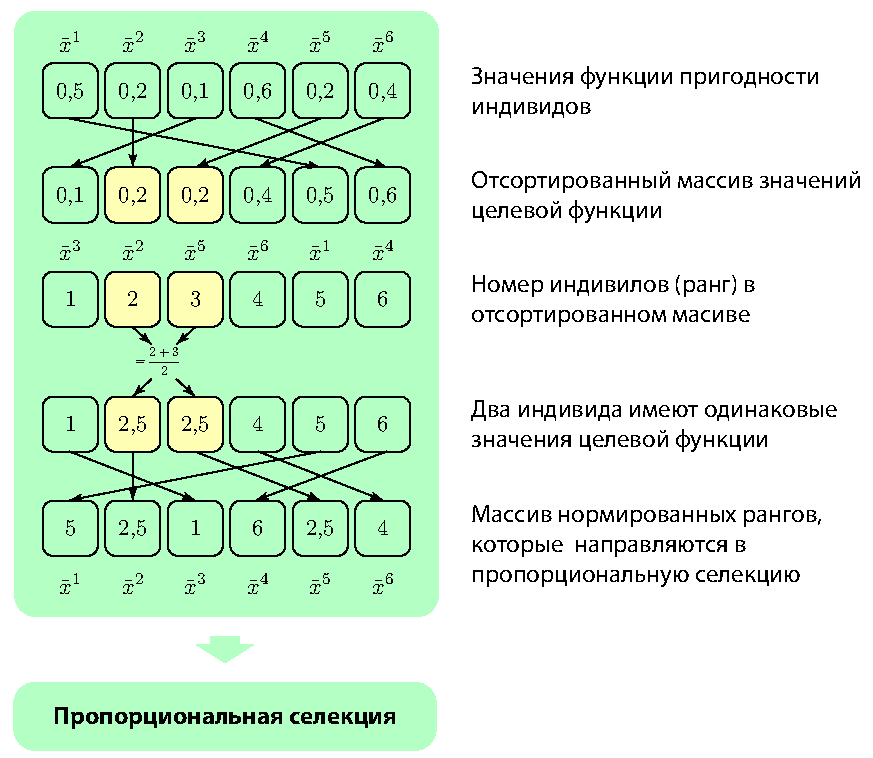
\includegraphics [scale=0.7] {RankSelection}
  \caption{Механизм работы ранговой селекции} 
  \label{SetOfOperatorsAlgorithms:img:RankSelection}  
\end{figure}

$ DataOfSel $ также не содержит каких-либо параметров относительно данного типа селекции.

Нет ограничений на множество задач оптимизации, которые может решать алгоритм оптимизации с данной селекцией.

В библиотеке \textbf{HarrixMathLibrary} данная селекция реализуется через функцию \textbf{MHL\_RankSelection}:

\href{https://github.com/Harrix/HarrixMathLibrary}{https://github.com/Harrix/HarrixMathLibrary}

\subsection{Турнирная селекция}\label{SetOfOperatorsAlgorithms:TournamentSelection}

Идентификатор: \textbf{TournamentSelection}.

Из популяции с равной вероятностью выбираются индивиды в количестве $ T $ (размер турнира), где $ 2\leq T\leq N $. При этом каждый индивид может попасть в группу (турнир) только один раз (турнирная селекция без возвращения). Из данной группы выбирается индивид с наибольшей пригодностью.

Значит, турнирная селекция определяется формулой:
\begin{align}
\label{SetOfOperatorsAlgorithms:eq:TournamentSelection}
Selection\left( Population, Fitness, DataOfSel\right) = \arg{\max_{\bar{x}\in H} {f_{fit}\left( \bar{x}\right) }}, \text{где }\\
H=\left\lbrace h^i | h_i=Random \left( Population/\left( \left\lbrace h^1\right\rbrace \cup \left\lbrace h^2\right\rbrace \cup \ldots  \cup \left\lbrace h^{i-1}\right\rbrace\right) \right) \right\rbrace, i=\overline{1,T}\nonumber.
\end{align}

Турнирная селекция является единственным типом данного оператора, который добавляет в $ DataOfSel $ дополнительный параметр – размер турнира $ T $. Обычно выбирают значение этого параметра равное $ T=2 $.

\textbf{Пример.} Массив возьмем тот же, что и в предыдущих примерах $ Fitness=\left\lbrace 0,5; 0,2; 0,1; 0,6; 0,2; 0,4\right\rbrace $. Размер турнира равен $ T=3 $. Пример работы оператора показан на рисунке:

\begin{figure} [h] 
  \center
  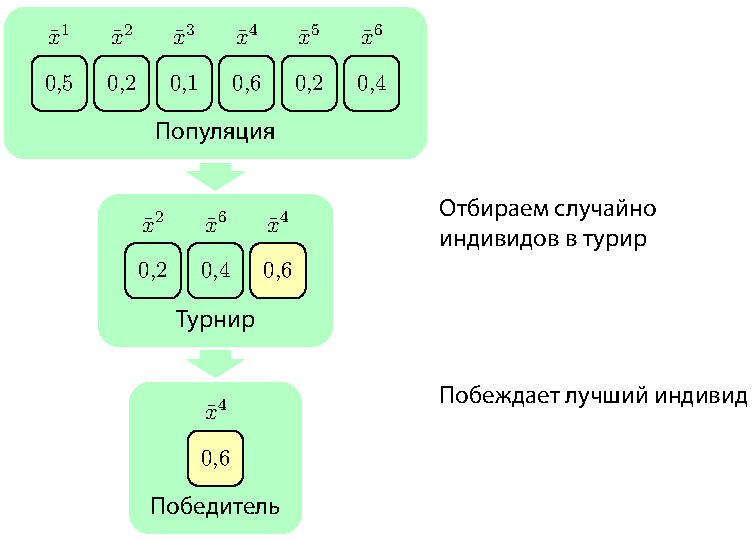
\includegraphics [scale=0.8] {TournamentSelection}
  \caption{Механизм работы турнирной селекции} 
  \label{SetOfOperatorsAlgorithms:img:TournamentSelection}  
\end{figure}

\begin{equation}
\label{SetOfOperatorsAlgorithms:eq:DataOfSel}
DataOfSel=\left( \begin{array}{c} TypeOfSel \\ T \end{array} \right).
\end{equation}

Нет ограничений на множество задач оптимизации, которые может решать алгоритм оптимизации с данной селекцией.

В библиотеке \textbf{HarrixMathLibrary} данная селекция реализуется через функцию \textbf{MHL\_TournamentSelection}:

\href{https://github.com/Harrix/HarrixMathLibrary}{https://github.com/Harrix/HarrixMathLibrary}

\section{Операторы скрещивания}\label{SetOfOperatorsAlgorithms:section_Crossover}

\textbf{Скрещивание (кроссовер)} --- оператор случайного формирования нового индивида из двух выбранных родителей с сохранением признаков обоих родителей.

\subsection{Одноточечное скрещивание}\label{SetOfOperatorsAlgorithms:SinglepointCrossover}

Идентификатор: \textbf{SinglepointCrossover}.

Данный оператор скрещивания используется для бинарных векторов.

Пусть имеется два родителя (родительские хромосомы) $ \overline{Parent}^1 $ и $ \overline{Parent}^2$. В случайном месте происходит разрыв между двумя позициями генов в обеих хромосомах. После этого хромосомы обмениваются частями, в результате чего образуются два потомка. Из них выбирается случайно один потомок, который и передается в качестве результата оператора скрещивания. То есть скрещивание происходит по формулам:

\begin{align}
\label{SetOfOperatorsAlgorithms:eq:SinglepointCrossover}
&Crossover \left( \overline{Parent}^1, \overline{Parent}^2, DataOfCros\right)=Random \left(\left\lbrace \overline{Offspring}^1; \overline{Offspring}^2\right\rbrace  \right), \\
&R=Random\left( \left\lbrace 2; 3; \ldots; n\right\rbrace \right); \nonumber \\
& \overline{Offspring}^1_i=\overline{Parent}^1_i, i=\overline{1,R-1};\nonumber\\
&  \overline{Offspring}^1_i=\overline{Parent}^2_i, i=\overline{R,n};\nonumber\\
&\overline{Offspring}^2_i=\overline{Parent}^2_i, i=\overline{1,R-1};\nonumber\\
& \overline{Offspring}^2_i=\overline{Parent}^1_i, i=\overline{R,n};\nonumber\\
&\overline{Offspring}^1\in X, \overline{Offspring}^2\in X.\nonumber
\end{align}

\textbf{Пример.} Для всех видов скрещивания будем использовать двух родителей: $\overline{Parent}^1\hmm={\left( 0; 1; 0; 1; 1; 1; 0; 0\right)}^\mathrm{T}  $ и $\overline{Parent}^2={\left( 1; 1; 0; 0; 1; 0; 1\right)}^\mathrm{T}  $. Одноточечное скрещивание показано на рисунке:

\begin{figure} [H] 
  \center
  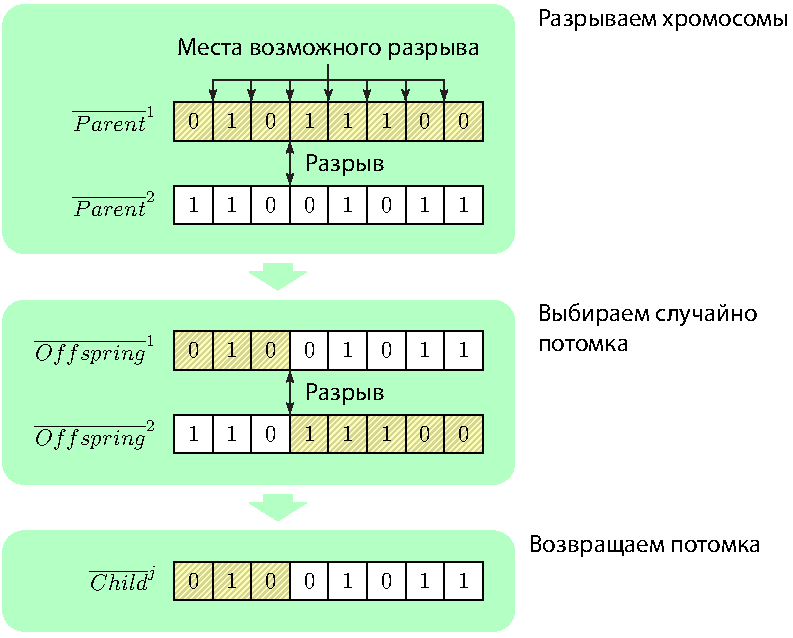
\includegraphics [scale=0.8] {SinglepointCrossover}
  \caption{Механизм работы одноточечного скрещивания} 
  \label{SetOfOperatorsAlgorithms:img:SinglepointCrossover}  
\end{figure}

$ DataOfCros $ не содержит каких-либо параметров относительно данного типа скрещивания.

В библиотеке \textbf{HarrixMathLibrary} данная селекция реализуется через функцию \textbf{TMHL\_SinglepointCrossover}:

\href{https://github.com/Harrix/HarrixMathLibrary}{https://github.com/Harrix/HarrixMathLibrary}

\subsection{Одноточечное скрещивание с возможностью полного копирования одного из родителей}\label{SetOfOperatorsAlgorithms:SinglepointCrossoverWithCopying}

Идентификатор: \textbf{SinglepointCrossoverWithCopying}.

Данный оператор скрещивания используется для бинарных векторов.

Отличается от стандартного одноточечного скрещивания тем, что точки разрыва могут происходить по краям родителей, что может привести к полному копированию родителя.

Пусть имеется два родителя (родительские хромосомы) $ \overline{Parent}^1 $ и $ \overline{Parent}^2$. В случайном месте происходит разрыв между двумя позициями генов в обеих хромосомах. После этого хромосомы обмениваются частями, в результате чего образуются два потомка. Из них выбирается случайно один потомок, который и передается в качестве результата оператора скрещивания. То есть скрещивание происходит по формулам:

\begin{align}
\label{SetOfOperatorsAlgorithms:eq:SinglepointCrossoverWithCopying}
&Crossover \left( \overline{Parent}^1, \overline{Parent}^2, DataOfCros\right)=Random \left(\left\lbrace \overline{Offspring}^1; \overline{Offspring}^2\right\rbrace  \right), \\
&R=Random\left( \left\lbrace 1; 3; \ldots; n+1\right\rbrace \right); \nonumber \\
& \overline{Offspring}^1_i=\overline{Parent}^1_i, i=\overline{1,R-1};\nonumber\\
&  \overline{Offspring}^1_i=\overline{Parent}^2_i, i=\overline{R,n};\nonumber\\
&\overline{Offspring}^2_i=\overline{Parent}^2_i, i=\overline{1,R-1};\nonumber\\
& \overline{Offspring}^2_i=\overline{Parent}^1_i, i=\overline{R,n};\nonumber\\
&\overline{Offspring}^1\in X, \overline{Offspring}^2\in X.\nonumber
\end{align}

\textbf{Пример.} Для всех видов скрещивания будем использовать двух родителей: $\overline{Parent}^1\hmm={\left( 0; 1; 0; 1; 1; 1; 0; 0\right)}^\mathrm{T}  $ и $\overline{Parent}^2={\left( 1; 1; 0; 0; 1; 0; 1\right)}^\mathrm{T}  $. Одноточечное скрещивание с возможностью полного копирования одного из родителей показано на рисунке:

\begin{figure} [H] 
  \center
  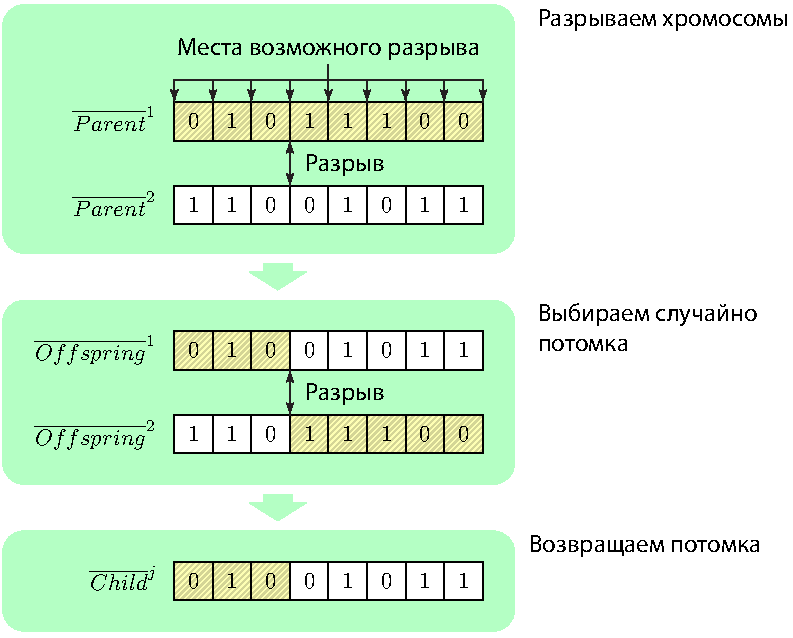
\includegraphics [scale=0.8] {SinglepointCrossoverWithCopying}
  \caption{Механизм работы одноточечного скрещивания с возможностью полного копирования одного из родителей} 
  \label{SetOfOperatorsAlgorithms:img:SinglepointCrossoverWithCopying}  
\end{figure}

$ DataOfCros $ не содержит каких-либо параметров относительно данного типа скрещивания.

В библиотеке \textbf{HarrixMathLibrary} данная селекция реализуется через функцию \textbf{TMHL\_SinglepointCrossoverWithCopying}:

\href{https://github.com/Harrix/HarrixMathLibrary}{https://github.com/Harrix/HarrixMathLibrary}

\subsection{Двухточечное скрещивание}\label{SetOfOperatorsAlgorithms:TwopointCrossover}

Идентификатор: \textbf{TwopointCrossover}.

Данный оператор скрещивания используется для бинарных векторов.

Пусть имеется два родителя (родительские хромосомы) $\overline{Parent}^1$ и $\overline{Parent}^2$. В двух случайных местах происходят разрывы между двумя позициями генов в обеих хромосомах. После этого хромосомы обмениваются частями, в результате чего образуются два потомка. Из них выбирается случайно один потомок, который и передается в качестве результата оператора скрещивания. То есть скрещивание происходит по формулам:

\begin{align}
\label{SetOfOperatorsAlgorithms:eq:TwopointCrossover}
&Crossover \left( \overline{Parent}^1, \overline{Parent}^2, DataOfCros\right)=Random \left(\left\lbrace \overline{Offspring}^1; \overline{Offspring}^2\right\rbrace  \right), \\
&r_1=Random\left( \left\lbrace 2; 3; \ldots; n\right\rbrace \right); \nonumber \\
&r_2=Random\left( \left\lbrace 2; 3; \ldots; n\right\rbrace \right); \nonumber \\
&R_1=\min \left( r_1, r_2\right) ; \nonumber \\
&R_2=\max \left( r_1, r_2\right) ; \nonumber \\
& \overline{Offspring}^1_i=\overline{Parent}^1_i, i=\overline{1,R_1-1};\nonumber\\
& \overline{Offspring}^1_i=\overline{Parent}^2_i, i=\overline{R_1,R_2-1};\nonumber\\
&  \overline{Offspring}^1_i=\overline{Parent}^1_i, i=\overline{R_2,n};\nonumber\\
& \overline{Offspring}^2_i=\overline{Parent}^2_i, i=\overline{1,R_1-1};\nonumber\\
& \overline{Offspring}^2_i=\overline{Parent}^1_i, i=\overline{R_1,R_2-1};\nonumber\\
&  \overline{Offspring}^2_i=\overline{Parent}^2_i, i=\overline{R_2,n};\nonumber\\
&\overline{Offspring}^1\in X, \overline{Offspring}^2\in X.\nonumber
\end{align}

\textbf{Пример.} Двухточечное скрещивание показано на рисунке:

\begin{figure} [H]
  \center
  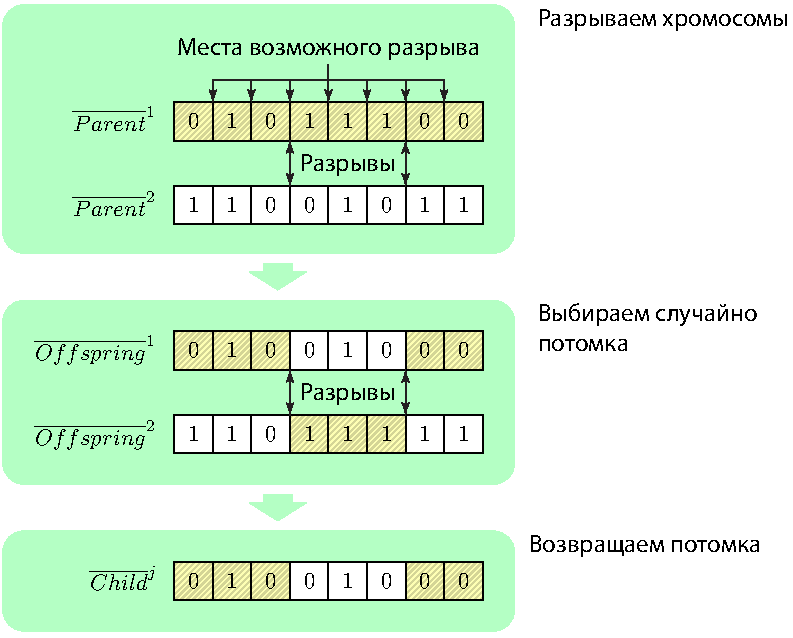
\includegraphics [scale=0.6] {TwopointCrossover}
  \caption{Механизм работы двухточечного скрещивания} 
  \label{SetOfOperatorsAlgorithms:img:TwopointCrossover} 
\end{figure}

$ DataOfCros $ не содержит каких-либо параметров относительно данного типа скрещивания.

В библиотеке \textbf{HarrixMathLibrary} данная селекция реализуется через функцию \textbf{TMHL\_TwopointCrossover}:

\href{https://github.com/Harrix/HarrixMathLibrary}{https://github.com/Harrix/HarrixMathLibrary}

\subsection{Двухточечное скрещивание с возможностью полного копирования одного из родителей}\label{SetOfOperatorsAlgorithms:TwopointCrossoverWithCopying}

Идентификатор: \textbf{TwopointCrossoverWithCopying}.

Данный оператор скрещивания используется для бинарных векторов.

Отличается от стандартного двухточечного скрещивания тем, что точки разрыва могут происходить по краям родителей, что может привести к полному копированию родителя.

Пусть имеется два родителя (родительские хромосомы) $\overline{Parent}^1$ и $\overline{Parent}^2$. В двух случайных местах происходят разрывы между двумя позициями генов в обеих хромосомах. После этого хромосомы обмениваются частями, в результате чего образуются два потомка. Из них выбирается случайно один потомок, который и передается в качестве результата оператора скрещивания. То есть скрещивание происходит по формулам:

\begin{align}
\label{SetOfOperatorsAlgorithms:eq:TwopointCrossoverWithCopying}
&Crossover \left( \overline{Parent}^1, \overline{Parent}^2, DataOfCros\right)=Random \left(\left\lbrace \overline{Offspring}^1; \overline{Offspring}^2\right\rbrace  \right), \\
&r_1=Random\left( \left\lbrace 1; 2; \ldots; n+1\right\rbrace \right); \nonumber \\
&r_2=Random\left( \left\lbrace 1; 2; \ldots; n+1\right\rbrace \right); \nonumber \\
&R_1=\min \left( r_1, r_2\right) ; \nonumber \\
&R_2=\max \left( r_1, r_2\right) ; \nonumber \\
& \overline{Offspring}^1_i=\overline{Parent}^1_i, i=\overline{1,R_1-1};\nonumber\\
& \overline{Offspring}^1_i=\overline{Parent}^2_i, i=\overline{R_1,R_2-1};\nonumber\\
&  \overline{Offspring}^1_i=\overline{Parent}^1_i, i=\overline{R_2,n};\nonumber\\
& \overline{Offspring}^2_i=\overline{Parent}^2_i, i=\overline{1,R_1-1};\nonumber\\
& \overline{Offspring}^2_i=\overline{Parent}^1_i, i=\overline{R_1,R_2-1};\nonumber\\
&  \overline{Offspring}^2_i=\overline{Parent}^2_i, i=\overline{R_2,n};\nonumber\\
&\overline{Offspring}^1\in X, \overline{Offspring}^2\in X.\nonumber
\end{align}

\textbf{Пример.} Двухточечное скрещивание с возможностью полного копирования одного из родителей показано на рисунке:

\begin{figure} [H]
  \center
  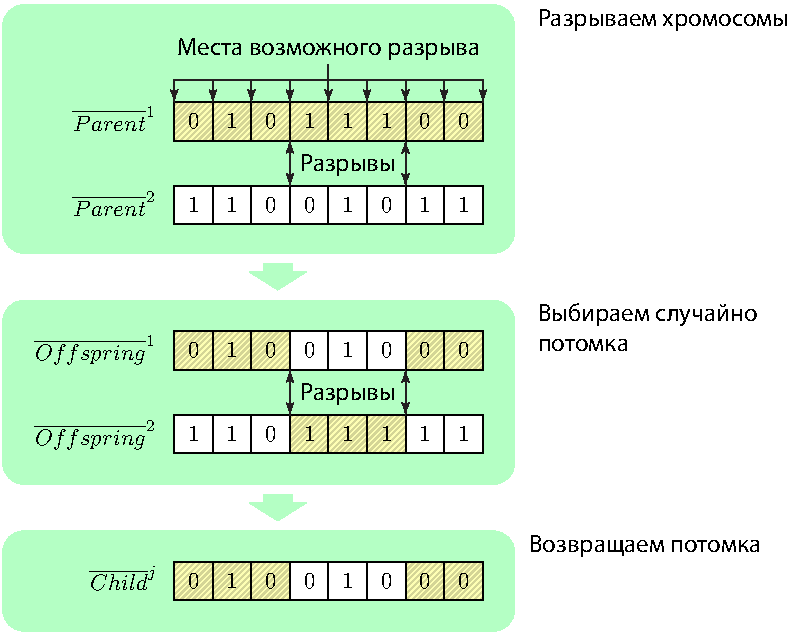
\includegraphics [scale=0.8] {TwopointCrossoverWithCopying}
  \caption{Механизм работы двухточечного скрещивания с возможностью полного копирования одного из родителей} 
  \label{SetOfOperatorsAlgorithms:img:TwopointCrossoverWithCopying} 
\end{figure}

$ DataOfCros $ не содержит каких-либо параметров относительно данного типа скрещивания.

В библиотеке \textbf{HarrixMathLibrary} данная селекция реализуется через функцию \textbf{TMHL\_TwopointCrossoverWithCopying}:

\href{https://github.com/Harrix/HarrixMathLibrary}{https://github.com/Harrix/HarrixMathLibrary}

\subsection{Равномерное скрещивание}\label{SetOfOperatorsAlgorithms:UniformCrossover}

Идентификатор: \textbf{UniformCrossover}.

Данный оператор скрещивания используется для бинарных векторов.

Пусть имеется два родителя (родительские хромосомы) $\overline{Parent}^1$ и $\overline{Parent}^2$. Потомок состоит из генов, каждый из которых выбран случайно из генов родителей на соответствующих позициях. То есть скрещивание происходит по формулам:

\begin{align}
\label{SetOfOperatorsAlgorithms:eq:UniformCrossover}
&Crossover \left( \overline{Parent}^1, \overline{Parent}^2, DataOfCros\right) = \overline{Offspring};\\
& \overline{Offspring}_i=Random\left( \left\lbrace \overline{Parent}^1_i;\overline{Parent}^2_i\right\rbrace \right), i=\overline{1,n} ;\nonumber\\
&\overline{Offspring}\in X.\nonumber
\end{align}

\textbf{Пример.} Равномерное скрещивание показано на рисунке:

\begin{figure} [H]
  \center
  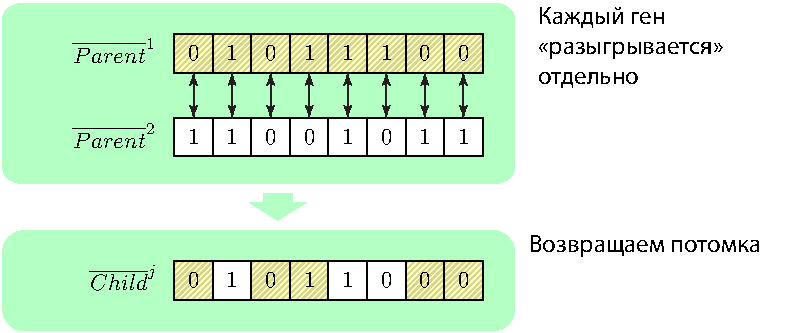
\includegraphics [scale=0.7] {UniformCrossover}
  \caption{Механизм работы равномерного скрещивания} 
  \label{SetOfOperatorsAlgorithms:img:UniformCrossover}  
\end{figure}

$ DataOfCros $ не содержит каких-либо параметров относительно данного типа скрещивания.

В библиотеке \textbf{HarrixMathLibrary} данная селекция реализуется через функцию \textbf{TMHL\_UniformCrossover}:

\href{https://github.com/Harrix/HarrixMathLibrary}{https://github.com/Harrix/HarrixMathLibrary}

\section{Операторы формирования нового поколения из родителей и потомков}\label{SetOfOperatorsAlgorithms:section_forming}

\textbf{Формирование нового поколения} --- оператор формирования нового поколения из массива родителей и получившихся потомков с использованием уже известных значений функции пригодности, как родителей, так и потомков.

\subsection{Только потомки}\label{SetOfOperatorsAlgorithms:OnlyOffspringGenerationForming}

Идентификатор: \textbf{OnlyOffspringGenerationForming}.

Данный оператор используется для векторов любой природы.

Данная схема предполагает формирование нового поколения из потомков и родителей таким, что в новое поколение попадают только потомки. Данный тип формирования нового поколения определяется формулой:
\begin{equation}
\label{SetOfOperatorsAlgorithms:eq:OnlyOffspringGenerationForming}
Forming \left( \begin{array}{c} Population\\MutChildPopulation\\Fitness\\FitnessOfMutChild\\DataOfForm\end{array}\right) =\left( \begin{array}{c} MutChildPopulation\\FitnessOfMutChild\end{array}\right).
\end{equation}

Здесь $ Population $ --- множество родителей, $MutChildPopulation$ --- множество потомков, $ Fitness $ -- множество значений целевой функции множества родителей, $ FitnessOfMutChild $ -- множество значений целевой функции множества родителей. 

$ DataOfForm $ не содержит каких-либо параметров относительно данного типа формирования нового поколения.


\subsection{Только потомки и копия лучшего индивида}\label{SetOfOperatorsAlgorithms:OnlyOffspringWithBestGenerationForming}

Идентификатор: \textbf{OnlyOffspringWithBestGenerationForming}.

Данный оператор используется для векторов любой природы.

Данная схема предполагает формирование нового поколения из потомков и родителей таким, что в новое поколение попадают только потомки (без одного) и копия лучшего индивида $ \overline{Best} $ (лучшего за всё время работы генетического алгоритма, а не только текущего поколения). В русской литературе данный способ часто называют селекцией элитизма. Данный тип формирования нового поколения определяется формулой:

\begin{align}
\label{SetOfOperatorsAlgorithms:eq:OnlyOffspringWithBestGenerationForming}
&Forming \left( \begin{array}{c} Population\\MutChildPopulation\\Fitness\\FitnessOfMutChild\\DataOfForm\end{array}\right) =\left( \begin{array}{c} \left\lbrace \bar{x}^i\right\rbrace \\\left\lbrace f^i\right\rbrace\end{array}\right),\\&\bar{x}^i=\left\lbrace \begin{aligned}
\overline{Best}&\text{, если }i=0; \\ \overline{MutChild}^i&\text{, если }i\neq 0;
\end{aligned}\right.\nonumber\\
&f_i=f\left( \bar{x}_i\right), i=\overline{1,N}.\nonumber
\end{align}

Здесь $ Population $ --- множество родителей, $MutChildPopulation$ --- множество потомков, $ Fitness $ -- множество значений целевой функции множества родителей, $ FitnessOfMutChild $ -- множество значений целевой функции множества родителей. 

$ DataOfForm $ не содержит каких-либо параметров относительно данного типа формирования нового поколения.


\section{Операторы <<малого>> изменения решения}\label{SetOfOperatorsAlgorithms:section_change}

\subsection{Мутация} \label{SetOfOperatorsAlgorithms:subsection_Mutation}

Идентификатор: \textbf{Mutation}.

Данный оператор используется для бинарных векторов.

\textbf{Мутация} --- оператор случайного изменения всех потомков из популяции. Цель данного оператора  не получить более лучшее решение, а разнообразить многообразие рассматриваемых индивидов. Обычно мутация предполагает незначительное изменение вектора. При выполнении оператора каждый ген каждого индивида с некоторой заданной вероятностью  $ ProbabilityOfMutation $ мутирует, то есть меняет свое значение на противоположное. Пусть у нас имеется некий бинарный вектор $ \overline{x} $.  Мутация происходит по формулам:
\begin{align}
\label{SetOfOperatorsAlgorithms:eq:Mutation}
&\overline{MutChild}_j=\left\lbrace \begin{aligned}
\overline{x}_j&\text{, если } random \left(0, 1 \right)>ProbabilityOfMutation; \\
1-\overline{x}_j&\text{, иначе }.
\end{aligned}\right.
\end{align}

Обычно в генетическом алгоритме вероятность мутации выбирается из трех вариантов: слабая ($ Weak $), средняя ($ Average $) и сильная ($ Strong $) мутация.
Отсюда вероятность мутации определяется формулой:
\begin{align}
\label{SetOfOperatorsAlgorithms:eq:ProbabilityOfMutation}
ProbabilityOfMutation\left( TypeOfMutation\right) =\\ =\left\lbrace \begin{aligned}
\frac{1}{3n}&\text{, если }TypeOfMutation=Weak; \\ \frac{1}{n}&\text{, если }TypeOfMutation=Average; \\ min\left(1, \frac{3}{n}\right) &\text{, если }TypeOfMutation=Strong.
\end{aligned}\right.\nonumber
\end{align}

Здесь
\begin{equation}
\label{SetOfOperatorsAlgorithms:eq:TypeOfMutation}
TypeOfMutation \in \left\lbrace Weak; Average;Strong\right\rbrace ,
\end{equation}

$ n $ --- длина вектора $ \bar{x}\in X $ бинарной задачи оптимизации.

В библиотеке \textbf{HarrixMathLibrary} данная селекция реализуется через функцию \textbf{TMHL\_MutationBinaryMatrix} (сразу мутируют все решения):

\href{https://github.com/Harrix/HarrixMathLibrary}{https://github.com/Harrix/HarrixMathLibrary}


% Список литературы
\addcontentsline{toc}{section}{Список литературы}
\bibliographystyle{utf8gost705u}  %% стилевой файл для оформления по ГОСТу
\bibliography{biblio}     %% имя библиографической базы (bib-файла)
\newpage

\end{document}